\documentclass[runningheads]{llncs}

% ---------- Packages ----------
\usepackage[T1]{fontenc}
\usepackage{graphicx}
\usepackage{amsmath,amssymb,amsfonts}
\usepackage{booktabs}
\usepackage{multirow}
\usepackage{url}
\usepackage{xcolor}
\usepackage{siunitx}
\usepackage{hyperref}
\usepackage{enumitem}
\usepackage{tikz}
\usetikzlibrary{arrows.meta,positioning,calc,fit}

\sisetup{detect-all=true}
\graphicspath{{figures/}{./}}

\begin{document}

\title{PatchTSTSpike: A Patch-Based Transformer Framework for Cloudburst-Like Extreme Rainfall Detection Using ERA5 Reanalysis}
\titlerunning{Rare-Event Detection of Cloudburst-Like Extreme Rainfall}

\author{Ankit Kumar\inst{1} \and Prashant Kumar\textsuperscript{*}\inst{1} \and Yukiharu Hiasaki\inst{2} \and Rajni\inst{3}}
\authorrunning{A. Kumar et al.}

\institute{
Department of Mathematics, National Institute of Technology Delhi, Delhi-110040, India\inst{1} \and
Department of Physics and Earth Sciences, Faculty of Science, University of the Ryukyus, Japan\inst{2} \and
Jindal Global Business School, O.P. Jindal Global University, Sonipat, Haryana-131001, India\inst{3} \\
\email{ankitx55@gmail.com, prashantkumar@nitdelhi.ac.in}
}



% \author{Ankit Kumar\inst{1}, Prashant Kumar\inst{2}}
% \authorrunning{A. Kumar and P. Kumar}

% \institute{
% Department of Applied Sciences, National Institute of Technology Delhi, India\\
% \email{ankitx55@gmail.com}
% \and
% Department of Applied Sciences, National Institute of Technology Delhi, India\\
% \email{prashantkumar@nitdelhi.ac.in}
% }



\maketitle

\begin{abstract}
The occurrence of cloudburst-like heavy rainfall events in the Himalayan region is very rare but highly destructive on the other hand predicting them is even more difficult, These event initiates from very complex atmospheric crossover like change in pressure, temperature, Wind etc. In this paper, we have developed PatchTST, that is, a custom spike aware temporal patch based transformer model. It is designed to analyze extreme rainfalls using ERA5 reanalysis data \cite{era5}. We evaluate the model using variable window length ranging from $30$ to $90$ days. Among all of these windows, the $30$-day look-back window provides the most promising detection performance, getting a $ROC$-$AUC$ of $0.6007$. While using longer temporal windows, particularly $60$ days, slight improvement in precision on the cost of reduced recall, implying a give and take between event detection sensitivity and prediction certainty. Overall, the used framework offers a subtle transformer-based approach for studying spike event like precipitation in mountains or hilly areas and provides a practical base for in-future data-driven research on Himalayan weather and it's extremes.
\keywords{Himalayan Meteorology \and Rare-Event Detection \and Transformer Models \and ERA5 Reanalysis \and Extreme Rainfall}
\end{abstract}



\section{Introduction}

Extreme rainfall events in the Himalayan region often cause severe floods and landslides \cite{li2018wh,chen2021nepal,dollan2024hma}. These events are difficult to model because they occur rarely and show strong seasonal variation. The low number of events also creates a strong class imbalance, which makes prediction challenging. In this paper, the problem is as a binary event detection using temporal data. Extreme rainfall days are defined using the threshold of month-wise 99th percentile of regional maximum precipitation.


\section{Related Work}

Almost all studies on Himalayan rainfall suggest that sudden change in pressure moves moisture and hills play an important role in producing extreme precipitation \cite{li2018wh,chen2021nepal,dollan2024hma}. However, The ERA5 Reanalysis datset such as struggles to capture accurately very localized mountain rainfall events \cite{era5,chen2021nepal,dollan2024hma}. To solve this problem, we use a more loacalized spike-detection approach based on extreme rainfall thresholds such as top 1 percentile. This allows proper identification of unusual rainfall conditions to long-term atmospheric records. An important difficulty in this dataset is the severe imbalance between normal and extreme events which is to be studied. To handle this, we use Focal Loss so that rare events are acknowledged during training rather than being normalized, like they do in every other model training \cite{focal}. We also apply Sharpness-Aware Minimization (SAM) to improve model stability and generalization \cite{sam}.


\section{Data and Preprocessing}

\subsection{Study Region}
The Himalayan region is characterized by surprisingly uneven terrains and strong monsoon-driven rainfall \cite{li2018wh,chen2021nepal,dollan2024hma}. These conditions generally leads to extreme event such as flash floods and landslides and cloudburst itself. In this paper, the entire Himalayan domain is treated as a single aggregated region. Our main target here is to detect those rarity.

\subsection{Predictor Set and Data Integrity}
Predictor variables are obtained from the daily ERA5(Climate Data Store) regional time series, It provide a consistent multi-decadal atmospheric trends and variations \cite{era5}. Five predictors are used: regional mean precipitation (\texttt{tp\_region\_mean\_mm}), near-surface temperature (\texttt{t2m\_region}), relative humidity (\texttt{r\_region}), wind component (\texttt{u\_region}), and total cloud cover (\texttt{tcc\_region}).

To avoid information leakage, the regional maximum precipitation (\texttt{tp\_region\_max\_mm}) is not used as an input feature. It is reserved only for constructing the target spike labels.

\subsection{Spike Label Construction}
Extreme rainfall detection is evaluated as a binary classification task, that is, Either a heavy rainfall or not, using setting a threshold on maximum daily precipitation series (\texttt{tp\_region\_max\_mm}). As we know rainfall patterns vary across seasons in the Himalayas, fixed thresholds are avoided in model training. Instead, spike events are defined using the month-wise 99th percentile threshold ($Q_{0.99}^{(m)}$).

A day $t$ is labeled as a rare event ($y_t=1$) if the maximum precipitation surpasses the threshold for that month respectively. Otherwise, it is labeled as a non-spike ($y_t=0$). This is how we have defined extreme rainfalls in our paper.

\begin{table}[t]
\caption{Class distribution in the training split. The positive spike class is extremely rare, making PR-AUC more informative than accuracy for model selection and evaluation.}
\label{tab:class_distribution_train}
\centering
\footnotesize
\setlength{\tabcolsep}{8pt}
\begin{tabular}{lcc}
\toprule
\textbf{Class} & \textbf{Count} & \textbf{Fraction} \\
\midrule
Non-spike (0) & 16,430 & 0.9886 \\
Spike (1)     & 189    & 0.0114 \\
\bottomrule
\end{tabular}
\end{table}

\begin{figure}[!t]
\centering

% ---------- Top row ----------
\begin{minipage}[t]{0.48\linewidth}
\centering

\includegraphics[width=\linewidth,valign=t]{study_area_clean_legend.png}

\vspace{1mm}
{\footnotesize (a) Study region covering the Himalayan domain used in this study.}
\end{minipage}
\hfill
\begin{minipage}[t]{0.48\linewidth}
\centering

\includegraphics[width=\linewidth,valign=t]{Distribution of Daily Regional Max Rainfall with Percentiles.png}

\vspace{1mm}
{\footnotesize (b) Distribution of regional maximum daily rainfall with key percentile thresholds.}
\end{minipage}

% ---------- Bottom row ----------
\begin{minipage}[t]{0.98\linewidth}
\centering

\includegraphics[width=\linewidth]{timeseries_tp_region_max_with_spikes.png}

\vspace{1mm}
{\footnotesize (c) Regional maximum daily precipitation time series with spike-day markers derived from month-wise P99 thresholding.}
\end{minipage}

\caption{Construction of cloudburst-like spike labels from the regional precipitation record. Panel (a) shows the Himalayan study region used for ERA5 aggregation. Panel (b) shows the upper-tail rainfall distribution used to define the spike threshold. Panel (c) shows the resulting spike-day markers on the regional maximum precipitation time series.}

\label{fig:spike_label_pipeline}

\end{figure}

% \begin{figure}[t]
% \centering
% 
\includegraphics[width=\linewidth]{timeseries_tp_region_max_with_spikes.png}
% \caption{Regional maximum daily precipitation time series with spike-day markers. Positive labels are defined using month-wise P99 thresholding of \texttt{tp\_region\_max\_mm}, so the marked days represent cloudburst-like rainfall spikes in the regional daily record.}
% \label{fig:tpmax_spike_timeseries}
% \end{figure}






% \subsection{Sequence Preparation and Feature Relevance}
% The regional predictor series is converted into overlapping windows of length $L \in \{30, 45, 60, 90\}$ to evaluate the impact of temporal context. Each sample is a tensor in $\mathbb{R}^{L \times 5}$ comprising consecutive daily observations. Prior to training, feature relevance was assessed on the training split using Pearson correlation, standardized mean separation, and mutual information. Analysis identifies regional mean precipitation (\texttt{tp\_region\_mean\_mm}) as the most significant predictor, followed by cloud cover (\texttt{tcc\_region}). While temperature, humidity, and wind-flow features show weaker standalone signals, they provide essential context within the integrated sequence model.

\section{Methodology}

\subsection{Sequence Construction}

The spike-detection problem is formulated as a binary classification task using daily regional atmospheric predictors. For a sequence length $L$, the model input is a tensor of multiple variable.
\[
X \in \mathbb{R}^{L \times F},
\]
where $F=5$ represents the number of predictor variables used in the non-leaky setup. Each sequence contains $L$ consecutive days of \texttt{tp\_region\_mean\_mm}, \texttt{t2m\_region}, \texttt{r\_region}, \texttt{u\_region}, and \texttt{tcc\_region}. The target corresponds to the binary spike label associated with the prediction time step.

To study the effect of temporal context, we evaluate four sequence lengths:
\[
L \in \{30, 45, 60, 90\}.
\]
These setup allow comparison between shorter and longer temporal windows under the same training setup. Every sequence is generated separately within the subsequent training, validation and test splits. It effectively ensures that no temporal leakage occurs between partitions.

\subsection{PatchTSTSpike Architecture}

\begin{figure*}[t]
\centering
\resizebox{\textwidth}{!}{%
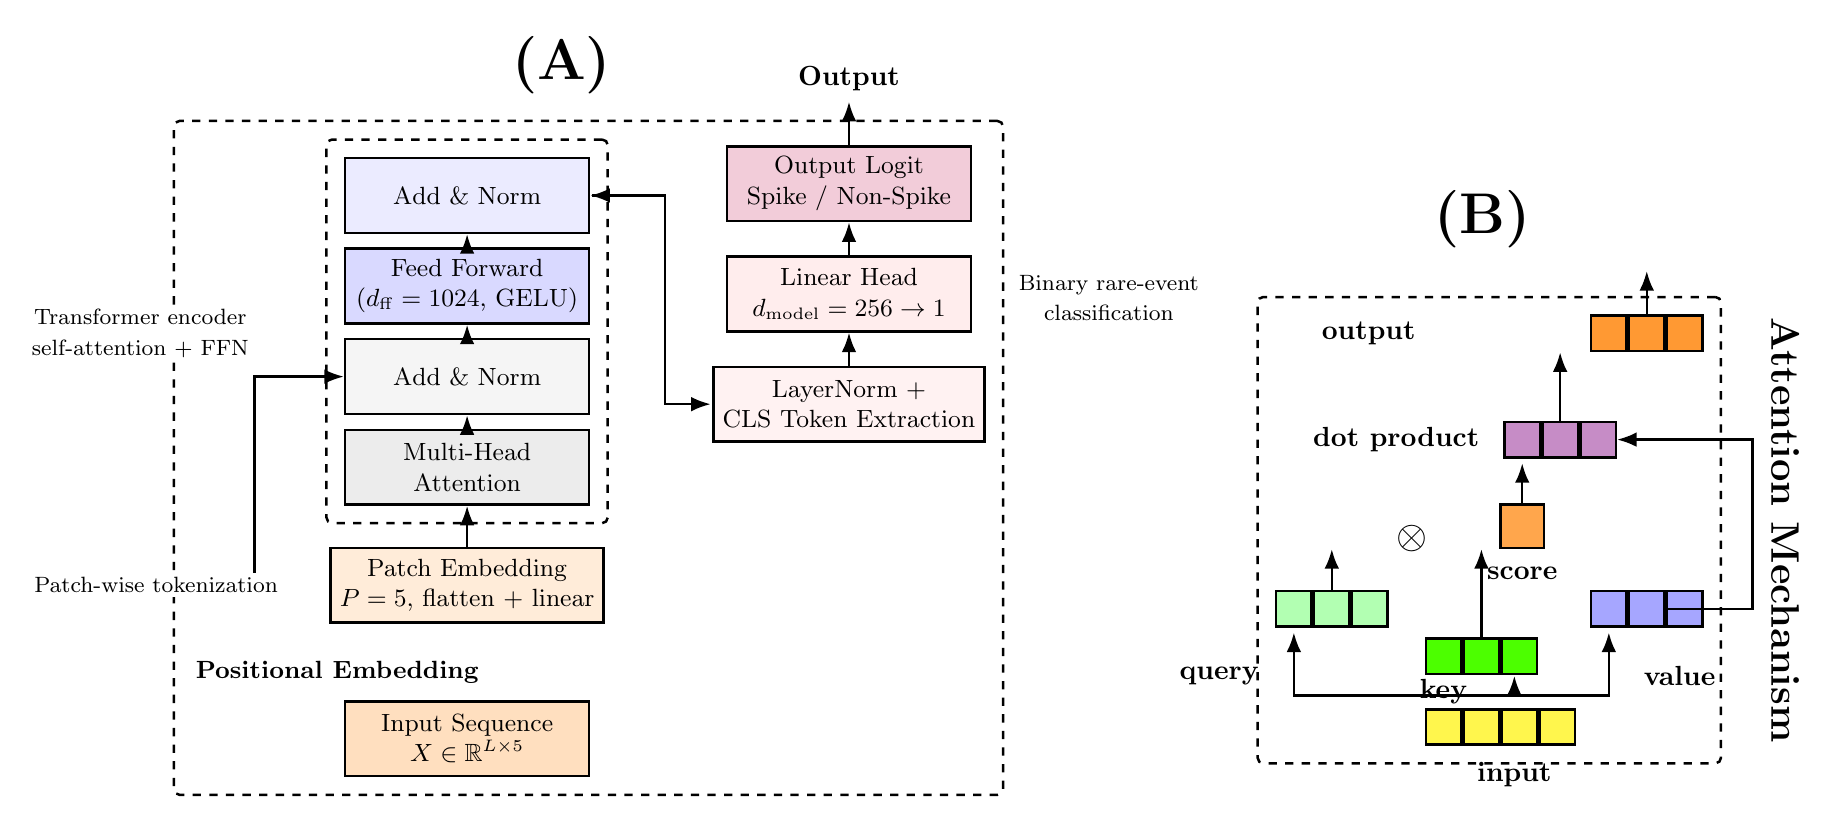
\begin{tikzpicture}[
    font=\small,
    >=Latex,
    line width=0.9pt,
    box/.style={
        draw,
        rectangle,
        minimum width=3.1cm,
        minimum height=0.95cm,
        align=center,
        fill=#1,
    },
    smallbox/.style={
        draw,
        rectangle,
        minimum width=2.2cm,
        minimum height=0.75cm,
        align=center,
        fill=#1,
    },
    token/.style={
        draw,
        rectangle,
        minimum width=0.45cm,
        minimum height=0.45cm,
        fill=#1
    },
    group/.style={
        draw,
        dashed,
        rounded corners=2pt,
        inner sep=0.22cm
    }
]

% =========================================================
% (A) PatchTSTSpike architecture
% =========================================================
\node[font=\bfseries\fontsize{22}{22}\selectfont] at (0,8.95) {(A)};

% Input
\node[box=orange!25] (input) at (-1.2,0.4) {Input Sequence\\$X \in \mathbb{R}^{L \times 5}$};

% positional embedding text moved
\node[font=\small\bfseries, fill=white, inner sep=1.2pt] (pe1txt) at (-2.85,1.25) {Positional Embedding};

% % plus and wave symbol aligned better
% \node[font=\LARGE] at (-0.15,1.18) {$\oplus$};

% little pos-encoding symbol moved near plus and aligned
% \draw[line width=1pt] (0.35,1.00) .. controls (0.50,1.30) and (0.70,1.30) .. (0.85,1.00);
% \draw[line width=1pt] (0.85,1.00) .. controls (1.00,0.70) and (1.20,0.70) .. (1.35,1.00);

% \draw[->] (input.north) -- (-1.2,1.00);

% patch embedding
\node[box=orange!15] (patch) at (-1.2,2.35) {Patch Embedding\\$P=5$, flatten + linear};

% arrow from positional/addition region to patch corrected
% \draw[->] (-0.15,1.40) -- (-0.15,2.05) -- (patch.south);

% encoder block stack with slightly more spacing
\node[box=gray!15] (mh1) at (-1.2,3.85) {Multi-Head\\Attention};
\node[box=gray!8]  (an1) at (-1.2,5.00) {Add \& Norm};
\node[box=blue!15] (ff1) at (-1.2,6.15) {Feed Forward\\($d_{\mathrm{ff}}=1024$, GELU)};
\node[box=blue!8]  (an2) at (-1.2,7.30) {Add \& Norm};

\draw[->] (patch.north) -- (mh1.south);
\draw[->] (mh1.north) -- (an1.south);
\draw[->] (an1.north) -- (ff1.south);
\draw[->] (ff1.north) -- (an2.south);

% residual paths adjusted so arrowheads sit better
\draw[->] ($(patch.west)+(-0.95,0)$) |- ($(an1.west)+(-0.30,0)$) -- (an1.west);
\draw[->] ($(an1.east)+(0.95,0)$) |- ($(an2.east)+(0.30,0)$) -- (an2.east);

% stack box
\node[group, fit=(mh1)(an1)(ff1)(an2)] (encfit) {};
% \node[font=\bfseries, rotate=90, fill=white, inner sep=1.2pt] at ($(encfit.west)+(-1.15,0)$) {$\times 4$};

% classifier head with slightly more spacing
\node[box=pink!20] (ln) at (3.65,4.65) {LayerNorm +\\CLS Token Extraction};
\node[box=pink!28] (linear) at (3.65,6.05) {Linear Head\\$d_{\mathrm{model}}=256 \rightarrow 1$};
\node[box=purple!20] (out) at (3.65,7.45) {Output Logit\\Spike / Non-Spike};

% arrows to head corrected
\draw[->] ($(an2.east)+(0.02,0)$) -- ++(0.93,0) |- ($(ln.west)+(-0.02,0)$);
\draw[->] (ln.north) -- (linear.south);
\draw[->] (linear.north) -- (out.south);
\draw[->] (out.north) -- ++(0,0.55) node[above,font=\bfseries] {Output};

% outer dashed panel for A
\node[group, fit=(input)(patch)(encfit)(ln)(linear)(out)(pe1txt)] {};

% annotations A moved as requested
\node[align=center, fill=white, inner sep=1.5pt] at (-5.15,2.35) {\footnotesize Patch-wise tokenization};
\node[align=center, fill=white, inner sep=1.5pt] at (-5.35,5.55) {\footnotesize Transformer encoder\\\footnotesize self-attention + FFN};
\node[align=center, fill=white, inner sep=1.5pt] at (6.95,6.00) {\footnotesize Binary rare-event\\\footnotesize classification};

% =========================================================
% (B) Attention mechanism
% =========================================================
\node[font=\bfseries\fontsize{22}{22}\selectfont] at (11.7,7.0) {(B)};

% input tokens
\node[token=yellow!70] (tin1) at (11.2,0.55) {};
\node[token=yellow!70, right=0cm of tin1] (tin2) {};
\node[token=yellow!70, right=0cm of tin2] (tin3) {};
\node[token=yellow!70, right=0cm of tin3] (tin4) {};
\node[font=\bfseries] at (12.1,-0.05) {input};

% Q K V
\node[token=green!30] (q1) at (9.3,2.05) {};
\node[token=green!30, right=0cm of q1] (q2) {};
\node[token=green!30, right=0cm of q2] (q3) {};
\node[font=\bfseries] at (8.35,1.2) {query};

\node[token=green!70!yellow] (k1) at (11.2,1.45) {};
\node[token=green!70!yellow, right=0cm of k1] (k2) {};
\node[token=green!70!yellow, right=0cm of k2] (k3) {};
\node[font=\bfseries] at (11.2,1.0) {key};

\node[token=blue!35] (v1) at (13.3,2.05) {};
\node[token=blue!35, right=0cm of v1] (v2) {};
\node[token=blue!35, right=0cm of v2] (v3) {};
\node[font=\bfseries] at (14.2,1.2) {value};

% score
\node[token=orange!70, minimum width=0.55cm, minimum height=0.55cm] (score) at (12.2,3.1) {};
\node[font=\bfseries] at (12.2,2.5) {score};

% dot product / weighted output / output
\node[token=violet!45] (dp1) at (12.2,4.2) {};
\node[token=violet!45, right=0cm of dp1] (dp2) {};
\node[token=violet!45, right=0cm of dp2] (dp3) {};
\node[font=\bfseries] at (10.6,4.2) {dot product};

\node[token=orange!80] (o1) at (13.3,5.55) {};
\node[token=orange!80, right=0cm of o1] (o2) {};
\node[token=orange!80, right=0cm of o2] (o3) {};
\node[font=\bfseries] at (10.25,5.55) {output};

% arrows B
\draw[->] (12.1,0.95) -- (12.1,1.2);
\draw[->] (12.1,0.95) -| (9.3,1.75);
\draw[->] (12.1,0.95) -| (13.3,1.75);

\draw[->] (q2.north) -- (q2.north |- score.south);
\draw[->] (k2.north) -- (k2.north |- score.south);
\node[font=\Large] at (10.8,2.95) {$\otimes$};

\draw[->] (score.north) -- (12.2,3.9);
\draw[->] (dp2.north) -- (dp2.north |- o2.south);

\draw[->] (v2.east) -- ++(1.1,0) |- (14.0,4.2) -- (dp3.east);

\draw[->] (o2.north) -- ++(0,0.55);

% attention panel box
\node[group, fit=(tin1)(tin4)(q1)(q3)(k1)(k3)(v1)(v3)(score)(dp1)(dp3)(o1)(o3)] (attfit) {};
\node[font=\bfseries\Large, rotate=270] at ($(attfit.east)+(0.8,0)$) {Attention Mechanism};

\end{tikzpicture}%
}
\caption{Architecture of the \textit{PatchTSTSpike} model. (A) The multivariate daily input sequence is divided into temporal patches, projected into an embedding space, processed by Transformer encoder layers, and mapped to a binary spike classification output. (B) Self-attention mechanism used within each encoder layer.}
\label{fig:patchtst_architecture}
\end{figure*}

To model multivariate atmospheric sequences, we use a transformer-based classifier called \textit{PatchTSTSpike}. The model reduces temporal redundancy by converting the input sequence into fixed-length temporal patches \cite{patchtst}.

For an input sequence $X \in \mathbb{R}^{L \times F}$, that sequence is divided into contiguous chunks  of length $P=5$. Let $N=L/P$ be the number of such chunks also called a patch. Each patch is flattened and sent directly into an embedded space:
\begin{equation}
z_i = W_p \,\mathrm{vec}(X_{(i-1)P+1:iP}) + b_p, \qquad z_i \in \mathbb{R}^{d},
\end{equation}
where $W_p$ and $b_p$ are learnable parameters and $d$ is the embedding dimension.

The patch embeddings are combined with a learnable classification token and positional embeddings:
\begin{equation}
\mathbf{H}_0 = [\mathbf{z}_{\mathrm{cls}}, z_1, z_2, \dots, z_N] + \mathbf{E}_{\mathrm{pos}}.
\end{equation}

The sequence is then processed by stacked Transformer encoder layers consisting of multi-head self-attention, residual connections, feed-forward networks, GELU activation, dropout, and layer normalization. The self-attention operation is defined as
\begin{equation}
\mathrm{Attn}(Q,K,V)=\mathrm{softmax}\left(\frac{QK^\top}{\sqrt{d_h}}\right)V,
\end{equation}
where $Q$, $K$, and $V$ are the query, key and the value projections.

After the encoder stack, the transformed token is extracted and passed through a linear layer to produce a scalar logit for spike classification. The main architecture settings are:

\begin{itemize}
\item embedding dimension (\texttt{d\_model}) = 256
\item attention heads (\texttt{n\_heads}) = 8
\item encoder layers (\texttt{n\_layers}) = 4
\item feed-forward dimension (\texttt{d\_ff}) = 1024
\item dropout = 0.1
\item patch length (\texttt{patch\_len}) = 5
\end{itemize}

Although inspired by patch-based transformer models for time-series data \cite{patchtst}, the architecture here is adapted specifically for rare rainfall spike detection rather than long-horizon forecasting.

\subsection{Training and Evaluation}

Model training uses focal loss to address the strong class imbalance, with validation PR-AUC used for model selection \cite{focal}. Optimization is performed using SAM with AdamW, some learning rate, weight decay of $10^{-4}$, batch size of 256, and 20 training epochs \cite{sam}. Mixed precision is disabled to maintain numerical stability.

Experiments are conducted for sequence lengths $L \in \{30,45,60,90\}$. When moving between window lengths, compatible weights are transferred while positional embeddings are reinitialized.

A good validation result is evaluated using ROC-AUC, PR-AUC, F1-score, precision, and recall. This way ensures that performance differences is observed due to the effect of temporal dependencies rather than changes in data splits or training configuration.

\section{Results and Discussion}


\begin{figure}[!t]
\centering

% ---------- Left image ----------
\begin{minipage}[t]{0.48\linewidth}
\centering

\includegraphics[width=\linewidth]{correlation_heatmap_nonleaky_train.png}

\vspace{1mm}
{\footnotesize (a) Correlation Heatmap}
\end{minipage}
\hfill
% ---------- Right image ----------
\begin{minipage}[t]{0.48\linewidth}
\centering

\includegraphics[width=\linewidth]{feature_relevance_nonleaky_train.png}

\vspace{1mm}
{\footnotesize (b) feature Comparison}
\end{minipage}

\label{fig:feature_analysis_combined}

\end{figure}

\subsection{Feature Relevance Analysis}

Using Pearson correlation we have depicted correlated variables, standardized mean separation, and mutual information (Table \ref{tab:feature_relevance}). Mean precipitation (\texttt{tp\_region\_mean\_mm}) shows the strongest relationship with Cloudburst, followed by cloud cover (\texttt{tcc\_region}). This shows that heavy dew or moisture and cloud covers are important factors related with extreme rainfall conditions.

Temperature (\texttt{t2m}), relative humidity (\texttt{r}), and wind (\texttt{u}) also contributed in the analysis but show weaker correlation. Overall, the analysis aligns with the chosen feature.

\begin{table}[t]

\label{tab:feature_relevance}
\label{tab:feature_summary}
\centering
\footnotesize
\setlength{\tabcolsep}{5pt}
\begin{tabular}{lccc}
\toprule
\textbf{Feature} & \textbf{Pearson with $y$} & \textbf{Effect Size} & \textbf{Mutual Info} \\
\midrule
\texttt{tp\_region\_mean\_mm} & 0.225925 & 1.543890 & 0.015254 \\
\texttt{tcc\_region}          & 0.052988 & 0.513079 & 0.001032 \\
\texttt{t2m\_region}          & 0.015824 & 0.156718 & 0.000389 \\
\texttt{r\_region}            & 0.006299 & 0.058178 & 0.000000 \\
\texttt{u\_region}            & -0.012699 & -0.123356 & 0.000000 \\
\bottomrule
\end{tabular}
\end{table}



\begin{figure}[t]
\centering

\includegraphics[width=\linewidth]{boxplots_top_features_nonleaky_train.png}
\caption{Boxplots of \texttt{tp\_region\_mean\_mm} and \texttt{tcc\_region}}
\label{fig:boxplots_top_features}
\end{figure}


\subsection{Temporal Context Performance}

We evaluated sliding windows of $30, 45, 60,$ and $90$ days. Among these settings, the $30$-day window shows the strongest overall result, achieving the highest test $PR$-$AUC$ ($0.0162$) and $ROC$-$AUC$ ($0.6007$). On the other hand, the $60$-day window produces higher precision and F1-score, behaving as a low level detector.

These results suggest that shorter temporal context ($L=30$) is better for capturing a wider range of spike events, while longer context ($L=60$) favors more confident predictions. Despite the difficulty of the task and the strong class imbalance, the results indicate that \textit{PatchTSTSpike} provides meaningful predictive capability for regional rainfall spike detection.


\begin{table}[t]
\caption{Window-length comparison for PatchTSTSpike.}
\label{tab:window_results}
\centering
\footnotesize
\setlength{\tabcolsep}{4pt}
\begin{tabular}{ccccccc}
\toprule
\textbf{$L$} & \textbf{Val PR-AUC} & \textbf{Test ROC-AUC} & \textbf{Test PR-AUC} & \textbf{Test F1} & \textbf{Precision} & \textbf{Recall} \\
\midrule
30 & 0.015253 & 0.600733 & 0.016226 & 0.041885 & 0.022099 & 0.400000 \\
45 & 0.059858 & 0.549670 & 0.012179 & 0.037037 & 0.022727 & 0.100000 \\
60 & 0.021638 & 0.544864 & 0.015355 & 0.047619 & 0.083333 & 0.033333 \\
90 & 0.019150 & 0.576554 & 0.012570 & 0.031915 & 0.017341 & 0.200000 \\
\bottomrule
\end{tabular}
\end{table}

% \begin{figure}[t]
% \centering
% 
\includegraphics[width=\linewidth]{window_length_comparison_nonleaky.png}
% \caption{Comparison of PatchTSTSpike performance across sequence lengths in the non-leaky setting. The figure shows test PR-AUC, test ROC-AUC, and test F1-score for $L=30$, $45$, $60$, and $90$.}
% \label{fig:window_length_comparison}
% \end{figure}

\begin{figure}[!t]
\centering

\begin{minipage}[t]{0.48\linewidth}
\centering

\includegraphics[width=\linewidth]{pr_curve_nonleaky_L30_test.png}

\vspace{1mm}
{\footnotesize (a) Precision--recall curve for the selected PatchTSTSpike model.}
\end{minipage}
\hfill
\begin{minipage}[t]{0.48\linewidth}
\centering

\includegraphics[width=\linewidth]{roc_curve_nonleaky_L30_test.png}

\vspace{1mm}
{\footnotesize (b) ROC curve for the selected PatchTSTSpike model.}
\end{minipage}

\caption{Final test-set behavior of the selected non-leaky PatchTSTSpike model with sequence length $L=30$. Panel (a) shows the precision--recall curve, while panel (b) shows the ROC curve.}
\label{fig:final_curves_l30}
\end{figure}

\section{Conclusion}

This study presents a framework for detecting Himalayan rainfall spikes using the custom \textit{PatchTSTSpike} transformer model. Extreme events are defined using month-wise 99th percentile thresholds, while atmospheric predictors are kept separate from the precipitation labels to avoid information leakage. The analysis shows that regional mean precipitation and cloud cover provide the strongest signals for identifying spike events, while temperature, humidity, and wind mainly offer supporting context. Experiments with different sequence lengths show that temporal context plays an important role. A 30-day window provides the most balanced performance, while a 60-day window produces fewer but more confident detections. Longer sequences appear to introduce additional noise that weakens the predictive signal.

Future work for our paper can be done by implementing this framework using the spatial information as well as the land–surface variables and snow cover to better capture atmospheric changes and variability.
\bibliographystyle{splncs04}
\begin{thebibliography}{8}

\bibitem{li2018wh}
Li, H., Beldring, S., Xu, C.-Y., Huss, M., Melvold, K., Jain, S.K.: 
Precipitation pattern in the Western Himalayas revealed by four datasets. 
Hydrology and Earth System Sciences \textbf{22}, 5097--5110 (2018)

\bibitem{chen2021nepal}
Chen, Y., Sharma, S., Zhou, X., Yang, K., Li, X., Niu, X.: 
Spatial performance of multiple reanalysis precipitation datasets on the southern slope of central Himalaya. 
Atmospheric Research \textbf{250}, 105365 (2021)

\bibitem{dollan2024hma}
Dollan, I.J., Bookhagen, B., Strecker, M.R., Thiede, R.C., Scherler, D.: 
An assessment of gridded precipitation products over High Mountain Asia. 
Journal of Hydrology: Regional Studies \textbf{54}, 101675 (2024)

\bibitem{era5}
Hersbach, H., Bell, B., Berrisford, P., et al.: The ERA5 global reanalysis. Quarterly Journal of the Royal Meteorological Society \textbf{146}(730), 1999--2049 (2020)

\bibitem{patchtst}
Nie, Y., Nguyen, N.H., Sinthong, P., Kalagnanam, J.: A time series is worth 64 words: Long-term forecasting with transformers. In: International Conference on Learning Representations (2023)

\bibitem{focal}
Lin, T.Y., Goyal, P., Girshick, R., He, K., Dollár, P.: Focal loss for dense object detection. In: Proceedings of the IEEE International Conference on Computer Vision, pp.~2980--2988 (2017)

\bibitem{sam}
Foret, P., Kleiner, A., Mobahi, H., Neyshabur, B.: Sharpness-aware minimization for efficiently improving generalization. In: International Conference on Learning Representations (2021)

\end{thebibliography}

\end{document}